\begin{tikzpicture}[rotate=-90, scale=6, font=\sffamily]
    \node[rotate=-90, scale=6] at (0, 0) {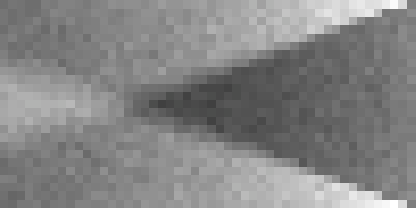
\includegraphics[width=1cm, height=.5cm, angle=-90]{figures/scintillator-yield-crop}};

    % coordinates of the colorbar
    \coordinate (A) at (.35, -.5);
    \coordinate (B) at (.35, .5);

    % draw the colorbar
    \draw[shade,left color=black!100,right color=black!0]
        ($(A) + (-.05, 0)$) rectangle (B);

    % draw the colorbar ticks and labels
	\foreach \i in {0, 20, ..., 100} {
	    \coordinate (C') at ($(A)!\i / 100!(B)$);
	    \draw (C') -- +(.75pt, 0);
	    \node[below=4pt] at (C') {\SI{\i}{\percent}};
    }

    % draw scintillator, fishtail and PMT
    \draw (-.25, .5) rectangle (.25, -.5);
    \draw[fill] (-.25, -.5) -- (-.02, -1.17) -- (.02, -1.17) -- (.25, -.5);
    \fill (-.02, -1.17) rectangle (.02, -1.37);
\end{tikzpicture}
